\section{Per-phase pipeline gallery}
\label{app:gallery}

This appendix walks through one concrete pass of the
\S\ref{sec:pipeline} pipeline on SO-101, showing the actual
artifact produced at each phase. All artifacts shown are reproduced
verbatim from the SO-101 run logged in
\texttt{artifacts/auto\_adapter\_from\_}\allowbreak\texttt{scratch\_so101\_artifacts/}
(referenced throughout the body of the paper).

\subsection{Phase 1: STUDY (parse MJCF, emit Spec)}

The agent reads \texttt{mjcf.xml}, identifies actuators and joints,
and writes a structured Spec object summarizing the robot's degrees
of freedom and limits. Excerpt:

\begin{lstlisting}[basicstyle=\ttfamily\scriptsize, frame=single, framerule=0pt,
    backgroundcolor=\color{gray!10}, columns=fullflexible, breaklines=true]
{
  "robot_id": "so101_from_scratch",
  "estimated_class": "arm",
  "dof": 5,
  "arm_joint_names": ["shoulder_pan", "shoulder_lift",
                      "elbow_flex", "wrist_flex", "wrist_roll"],
  "joint_limits": {
    "shoulder_pan":   [-1.92, 1.92],
    "shoulder_lift":  [-1.75, 1.75],
    "elbow_flex":     [-1.69, 1.69],
    "wrist_flex":     [-1.66, 1.66],
    "wrist_roll":     [-2.74, 2.84]
  },
  "ee_site": "ee_site",
  "ee_body": "gripper_link",
  "gripper_actuator_names": ["act_jaw_visual"],
  "actuator_type_hint": "position"
}
\end{lstlisting}

\subsection{Phase 2: GENERATE (Spec $\rightarrow$ driver code)}

The agent emits \texttt{driver\_from\_scratch.py}: 546 lines of
self-contained Python that exposes \texttt{home}, \texttt{move\_cartesian},
\texttt{gripper\_open}, \texttt{gripper\_close}, etc. The
inverse-kinematics inner loop, written by the agent without any
skeleton library, is reproduced below:

\begin{lstlisting}[basicstyle=\ttfamily\scriptsize, frame=single, framerule=0pt,
    backgroundcolor=\color{gray!10}, columns=fullflexible, breaklines=true,
    language=Python]
for iteration in range(max_iter):
    self.set_joint_positions(q)
    mujoco.mj_forward(self.model, self.data)
    current_xyz = self.data.site_xpos[self.site_id].copy()
    error = target_xyz - current_xyz
    if np.linalg.norm(error) < tol:
        return q, True, np.linalg.norm(error)

    J = self.compute_jacobian()
    # Adaptive damping: scales with error magnitude
    lambda_damping = self.ik_lambda_base * (1.0 + np.linalg.norm(error))
    JtJ = J.T @ J + lambda_damping**2 * np.eye(self.n_joints)
    dq = np.linalg.solve(JtJ, J.T @ error)
    # Step-size control prevents overshoot in poorly-conditioned regions
    step = min(1.0, 0.5 / (np.linalg.norm(dq) + 1e-6))
    q += step * dq
    q = self._clamp_to_limits(q)
\end{lstlisting}

Damped Least Squares with adaptive $\lambda$ and step-size clamping
is a textbook IK formulation, here written from scratch by the
agent against the per-robot Spec produced in Phase~1. The choice
is deliberate rather than a limitation: DLS stays well-behaved
near singularities and needs nothing beyond \texttt{numpy},
matching the self-contained delivery constraint (\S\ref{sec:modes}).

\subsection{Phase 3: VALIDATE (run the harness)}

The driver is imported and exercised against a fixed,
robot-class-aware test suite. SO-101's seven tests are reproduced
verbatim from \texttt{validate\_report.json} in Table~\ref{tab:validate}:

\begin{table}[H]
\centering
\small
\begin{tabular}{llr}
\toprule
\textbf{Test} & \textbf{Status} & \textbf{Metric} \\
\midrule
no\_skeleton\_import  & OK & --- \\
robot\_class\_present & OK & --- \\
build\_from\_mjcf     & OK & --- \\
home                  & OK & --- \\
ik\_roundtrip         & OK & 9.67\,mm err \\
gripper\_cycle        & OK & --- \\
describe              & OK & --- \\
\bottomrule
\end{tabular}
\caption{SO-101 validate-phase output (7/7); exact contents of
\texttt{artifacts/.../validate\_report.json}.}
\label{tab:validate}
\end{table}

If any test fails, the orchestrator re-enters Phase~2 with the
failure surfaced as a structured error in the prompt
(Appendix~\ref{app:reliability} reports the controlled rerun showing the
loop converges at outer iteration~1 on SO-101).

\subsection{Phase 4: EXPORT (package the artifact)}

A directory snapshot is captured for downstream consumption. The
SO-101 artifact tree:

\begin{lstlisting}[basicstyle=\ttfamily\scriptsize, frame=single, framerule=0pt,
    backgroundcolor=\color{gray!10}, columns=fullflexible]
artifacts/auto_adapter_from_scratch_so101_artifacts/
|-- driver_from_scratch.py    # 546 lines, agent-written
|-- mjcf.xml                  # symlink to assets/mjcf/so101_*.xml
|-- study.json                # Phase 1 output (Spec)
|-- validate_report.json      # Phase 3 output (test results)
\-- IMPLEMENTATION_SUMMARY.md # agent-written narrative
\end{lstlisting}

\subsection{Phase 5: DEMO (rendered execution)}

The exported driver is exercised by a small demo script (\texttt{home()}
then a reach target then \texttt{home()}) and the rollout is rendered
frame by frame. Figure~\ref{fig:demo-frame} shows the rollout at
the moment the end-effector reaches its target. The
full filmstrip for this same task is row (a) of
Figure~\ref{fig:filmstrips} in Appendix~\ref{app:filmstrips};
Appendix~\ref{app:traces} gives a side-by-side Auto-Adapter vs.\
Code-as-Policies trace for one task.

\begin{figure}[H]
\centering
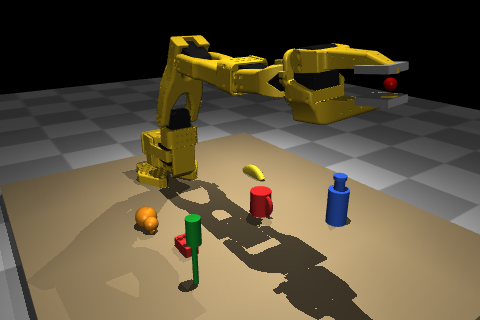
\includegraphics[width=0.7\columnwidth]{figures/film_so101_reach_3.png}
\caption{SO-101 demo frame at \texttt{reach\_x+5} target position
(end-effector at home$+5$\,cm in X, in MuJoCo). The synthesized
driver's \texttt{move\_cartesian} produced the trajectory. Compare
against Figure~\ref{fig:filmstrips}(a) for the full rollout.}
\label{fig:demo-frame}
\end{figure}
